% Completa los datos convenientemente en las zonas marcadas con TODO

\documentclass{beamer}
%PARA VISUALIZAR PRESENTACIONN CON NOTAS USAR VISUALIZADOR "pdfpc":
%Para ver las notas, el cronometro y siguente diapo:
% pdfpc --notes=right slides.pdf
% "tecla p": para pausar el cronometro
\mode<presentation> {
  \usetheme{CambridgeUS}
  \usecolortheme{crane} % color naranja
}

\definecolor{mypink}{RGB}{250,181,235}
\definecolor{mygreen}{RGB}{186, 242, 187}
\definecolor{mymint}{RGB}{186, 242, 216}
\definecolor{myred}{RGB}{236, 64, 103}

\setbeamercolor*{structure}{bg=mypink!20,fg=mypink}

\setbeamercolor*{palette primary}{use=structure,fg=white,bg=structure.fg}
\setbeamercolor*{palette secondary}{use=structure,fg=white,bg=structure.fg!75} %fondo de abajo en medio
\setbeamercolor*{palette tertiary}{use=structure,fg=white,bg=black} %fondo de la izquierda
%\setbeamercolor*{palette quaternary}{fg=white,bg=black}

%\setbeamercolor{section in toc}{fg=black,bg=white}
\setbeamercolor{alerted text}{use=structure,fg=structure.fg!50!black!80!black}

%\setbeamercolor{titlelike}{parent=palette primary,fg=structure.fg!50!black}
\setbeamercolor{frametitle}{bg=mypink!85,fg=white} %Barra de titulo (contenidos, etc)

\setbeamercolor*{titlelike}{use=structure,fg=black,bg=mypink!70}
\setbeamercolor{item projected}{fg=black,bg=mypink}

%\definecolor{mypink}{RGB}{250,181,235}
%\setbeamercolor*{structure}{bg=mypink!20,fg=mypink}

%\setbeamercolor*{palette primary}{use=structure,fg=white,bg=structure.fg}
%\setbeamercolor*{palette secondary}{use=structure,fg=white,bg=structure.fg!75}


%\setbeamercolor{titlelike}{parent=structure,bg=mypink,fg=structure.fg!50!black}
%\setbeamercolor{frametitle}{bg=mypink!85,fg=white}
%\setbeamercolor{section in toc}{fg=black,bg=white}

%\setbeamercolor{titlelike}{parent=structure,bg=mypink} % Cambia el color de la caja del título de la página inicial

\setbeamertemplate{navigation symbols}{} % ocultar iconos de navegación
\setbeamerfont{subsection in toc}{size=\small} % reducir tamaño en TOC
\setbeamerfont{date}{size=\tiny}
\usepackage[spanish]{babel}
\usepackage[utf8]{inputenc}
\usepackage{graphicx}
\usepackage{booktabs}
\usepackage{hyperref}
\usepackage{multicol}
\usepackage{pgfpages}
\usepackage{listings}
\usepackage{multimedia}
\usepackage[export]{adjustbox}
\usepackage{outlines} % Para poner bullets tabulados (\1 \2 \3 ...) y no items

\usepackage{array,tabularx} % para tabular leyenda de ecuaciones
\newenvironment{conditions*} % entorno de "leyenda de ecuación"
  {\par\vspace{\abovedisplayskip}\noindent
   \tabularx{\columnwidth}{>{$}l<{$} @{\ : } >{\raggedright\arraybackslash}X}}
  {\endtabularx\par\vspace{\belowdisplayskip}}
  
% USO DE NOTAS
%\setbeameroption{show notes} % Para mostrar u ocultar (hide/show)
%\setbeameroption{show only notes} % Mostrar solo las notas
%\setbeameroption{show notes on second screen=right} % Mostrar notas en otra pantalla
\setbeamertemplate{note page}{ % asi solo muestro el texto de las notas
  \insertnote%
}

%========= TODO: datos internos del documento
\hypersetup{
	pdftitle={Defensa de trabajo de fin de grado de Isabel Cebollada Gracia},
	pdfauthor={Isabel Cebollada Gracia},
	pdfsubject={Sistema de monitorización para el control y estudio del bienestar de animales de laboratorio mediante una infraestructura de bajo coste},
	pdfkeywords={raspberry, inteligencia artificial, machine learning, deep learning, visión artificial},
	pdfproducer={pdfLaTeX},
  colorlinks=true,
  linkcolor=blue
}
%=========

%========= TODO: diapositiva de portada
\title[Sistema de monitorización]{Sistema de monitorización para el control y estudio del bienestar de animales de laboratorio mediante una infraestructura de bajo coste} % El título reducido aparece en la parte inferior de todas las diapositivas
                                         % El título completo aparece solo en la diapositiva de portada
\author[Isabel Cebollada Gracia]{Isabel Cebollada Gracia}
\institute[URJC]
{
\textit{\href{mailto:i.cebollada.2018@alumnos.urjc.es}{\color{blue}{\underline{i.cebollada.2018@alumnos.urjc.es}}}}\\
\vspace{0.5cm}

\includegraphics[width=3cm]{figs/logo-urjc}\\
\vspace{1cm}
Trabajo fin de grado
}
\date{5 de julio de 2022}
%=========

%========= COMIENZO DEL DOCUMENTO
\begin{document}

%========= Portada inicial con notas
\begin{frame}[plain] % plain: quita header y footer
\large{\titlepage}
\note[item]{En esta presentación voy a hablar sobre mi trabajo de fin de grado, que consiste en la creación de un sistema}
\note[item]{CONTROL Y ESTUDIO DEL BIENESTAR DE ANIMALES}
\end{frame}

%========= Licencia
\begingroup
\hypersetup{linkcolor=white}
\begin{frame}
% Este diseño se corresponde con la licencia CC-BY-NC-SA.
% Por supuesto, puedes poner la licencia que mejor se adapte al propósito de tu trabajo.
% Recuerda que, si no se especifica ninguna licencia, esta -como cualquier creación artística- pasaría a estar licenciada con todos los derechos reservados (copyright).

\cleardoublepage

\begin{figure}
 \ \ \ \ 
\includegraphics[width=0.25\linewidth]{figs/by-nc-sa.png}
 \label{fig:cc} 
 \end{figure}

\

\

\

\noindent
Este trabajo se distribuye bajo los términos de la licencia internacional \href{http://creativecommons.org/licenses/by-nc-sa/4.0/}{CC BY-NC-SA International License} (Creative Commons AttributionNonCommercial-ShareAlike 4.0). Usted es libre de \textit{(a) compartir}: copiar y redistribuir el material en cualquier medio o formato; y \textit{(b) adaptar}: remezclar, transformar y crear a partir del material. El licenciador no puede revocar estas libertades mientras cumpla con los términos de la licencia:

\begin{itemize}
\item \textit{Atribución}. Usted debe dar crédito de manera adecuada, brindar un enlace a la licencia, e indicar si se han realizado cambios. Puede hacerlo en cualquier forma razonable, pero no de forma tal que sugiera que usted o su uso tienen el apoyo de la licenciante.
\item \textit{No comercial}. Usted no puede hacer uso del material con propósitos comerciales.
\item \textit{Compartir igual}. Si remezcla, transforma o crea a partir del material, debe distribuir su contribución bajo la la misma licencia del original.
\end{itemize}

\begin{flushright}
		\vspace{7.0 cm}
		\emph{Documento de} \textbf{Isabel Cebollada}. % TODO: pon aquí tu nombre cuando hagas el documento
\end{flushright}


\end{frame}
\endgroup

%========= Índice o tabla de contenidos (TOC)
\begin{frame}
\frametitle{Contenidos}
%\begin{multicols}{2} % si tengo muchas secciones, lo parte en dos columnas
  \tableofcontents[hideallsubsections] % no muestra subsecciones
%\end{multicols}
\note[item]{La presentación esta dividida en cinco partes.}
\end{frame}

\begingroup
\hypersetup{linkcolor=white}
%========= Diapositiva "vacía" de comienzo de sección:
\section*{}
\begin{frame}{}
  \centering \Huge
  \emph{Introducción}
\note[item]{Comencemos con la introducción a la robótica.}
\end{frame}

\section{Introducción}
\subsection{Contexto del trabajo}
%========= Diapositiva con imágenes:
\begin{frame}
\frametitle{Introducción a la robótica}
¿Qué es la robótica?
\begin{itemize}
\item Campo de investigación muy importante que continua en desarrollo.
\item Objetivo: Realizar trabajos \textcolor{myred}{aburridos} o \textcolor{myred}{peligrosos} para el humano.
\end{itemize}
\note[item]{La robótica es un campo de investigación muy importante en la actualidad que continua en desarrollo.}
\note[item]{Aburridos}
\note[item]{Sucios}
\note[item]{Peligrosos}
\note[item]{}
\note[item]{Para entender el concepto de robótica es necesario comprender qué es un robot.}
\end{frame}

\begin{frame}
\frametitle{Definición de robot}
¿Qué es un robot?
\begin{figure}
\centering
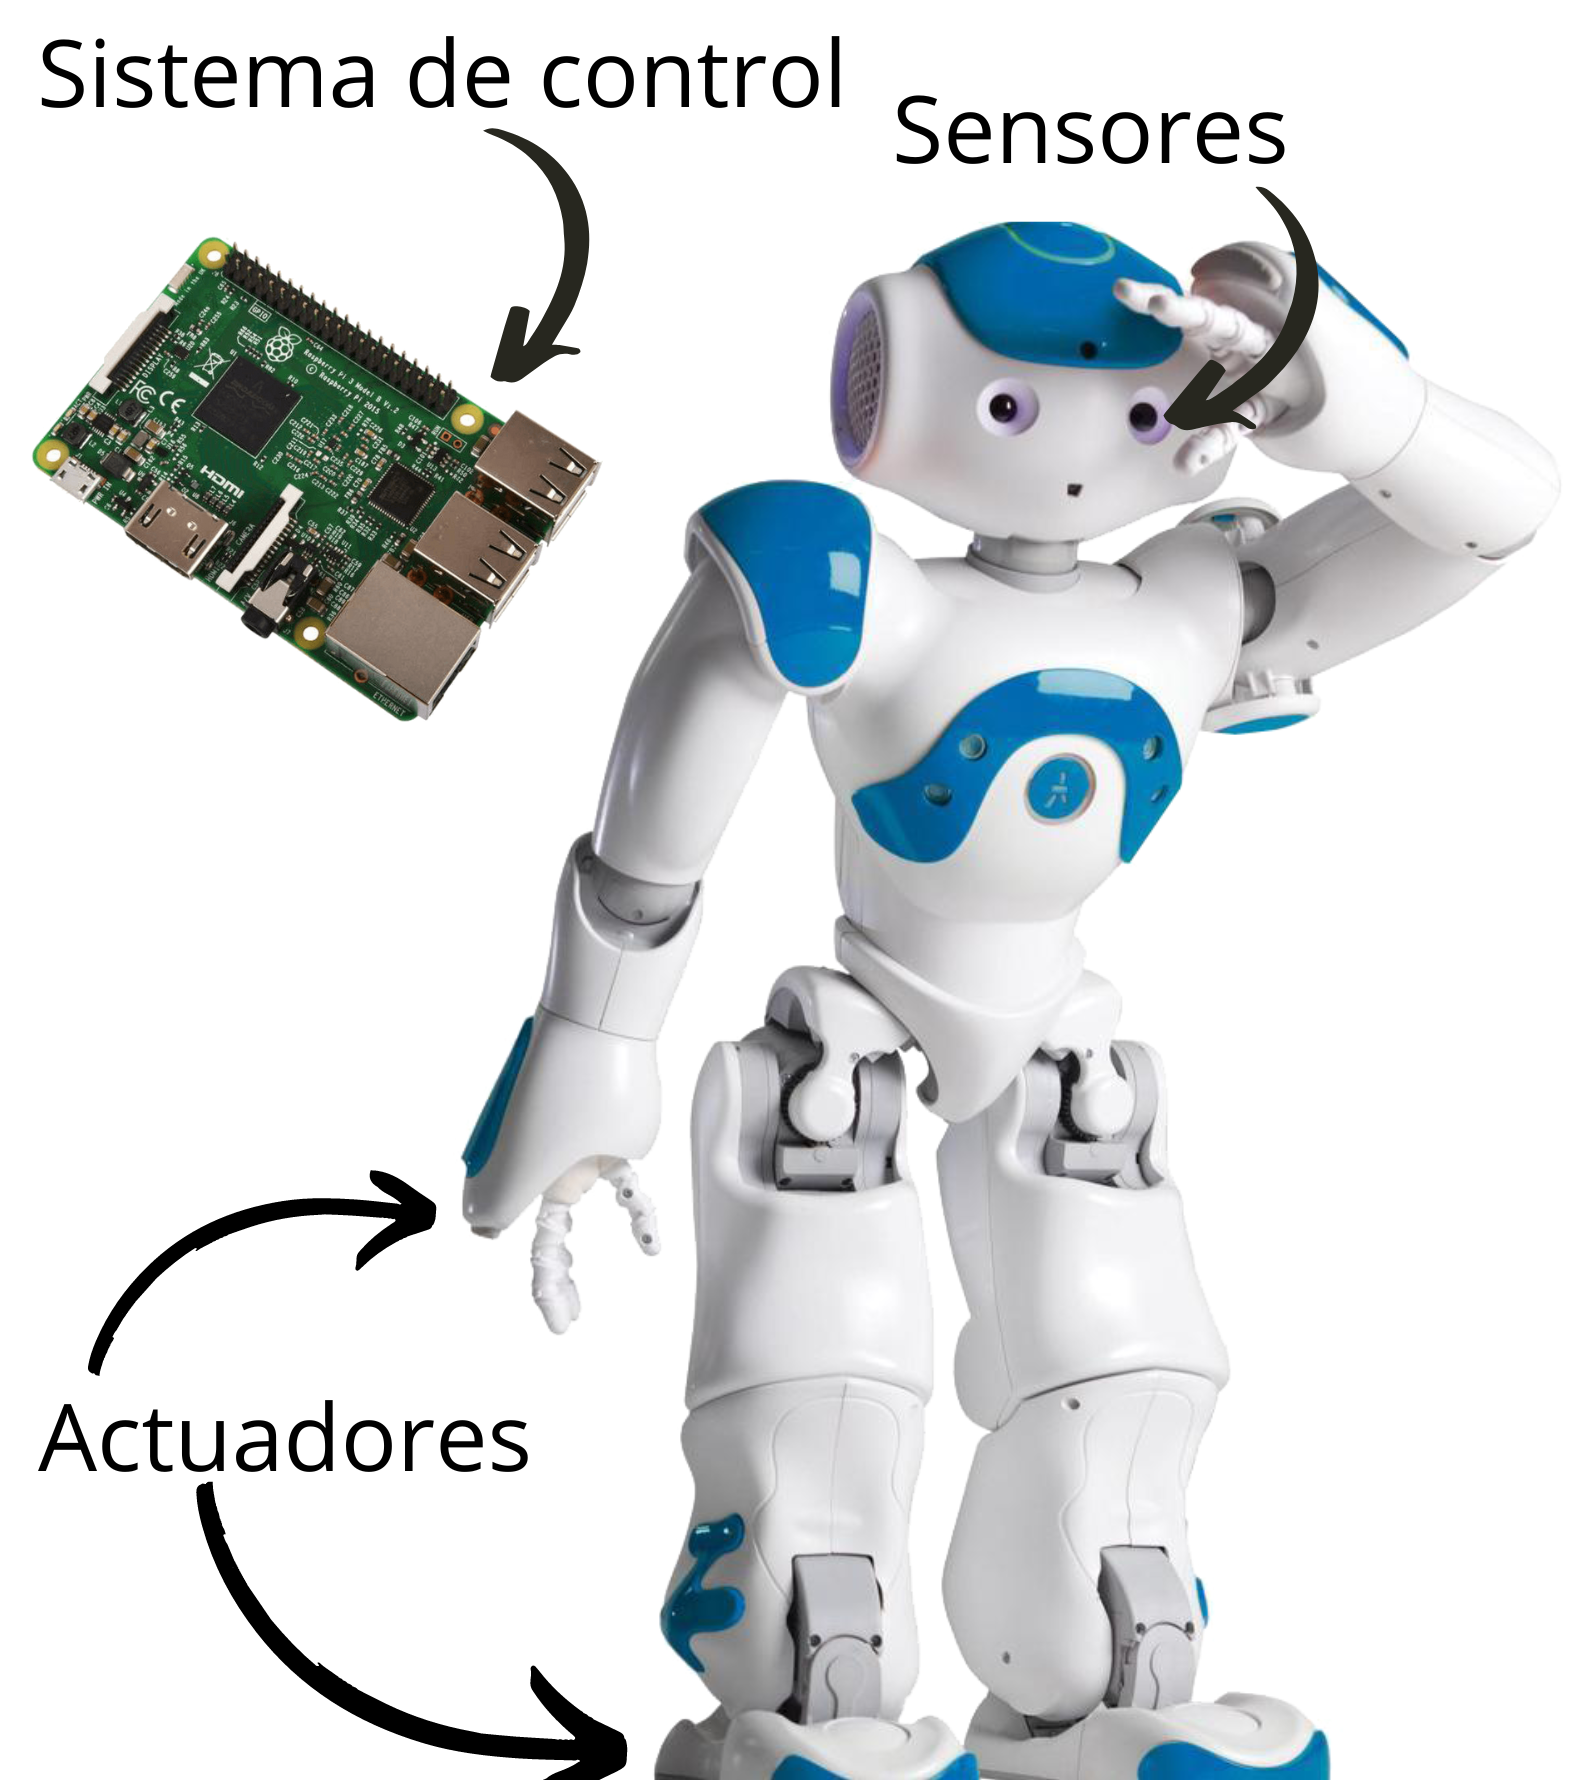
\includegraphics[width=6cm]{figs/robot}
\end{figure}
\note[item]{A lo largo de los años el concepto de robótica ha ido variando, así como la definición de robot. Actualmente, se entiende por robot a cualquier dispositivo dotado por sensores, actuadores y un sistema de control.}
\end{frame}

\begin{frame}
\frametitle{Algunos tipos de sensores}
\begin{figure}
\centering
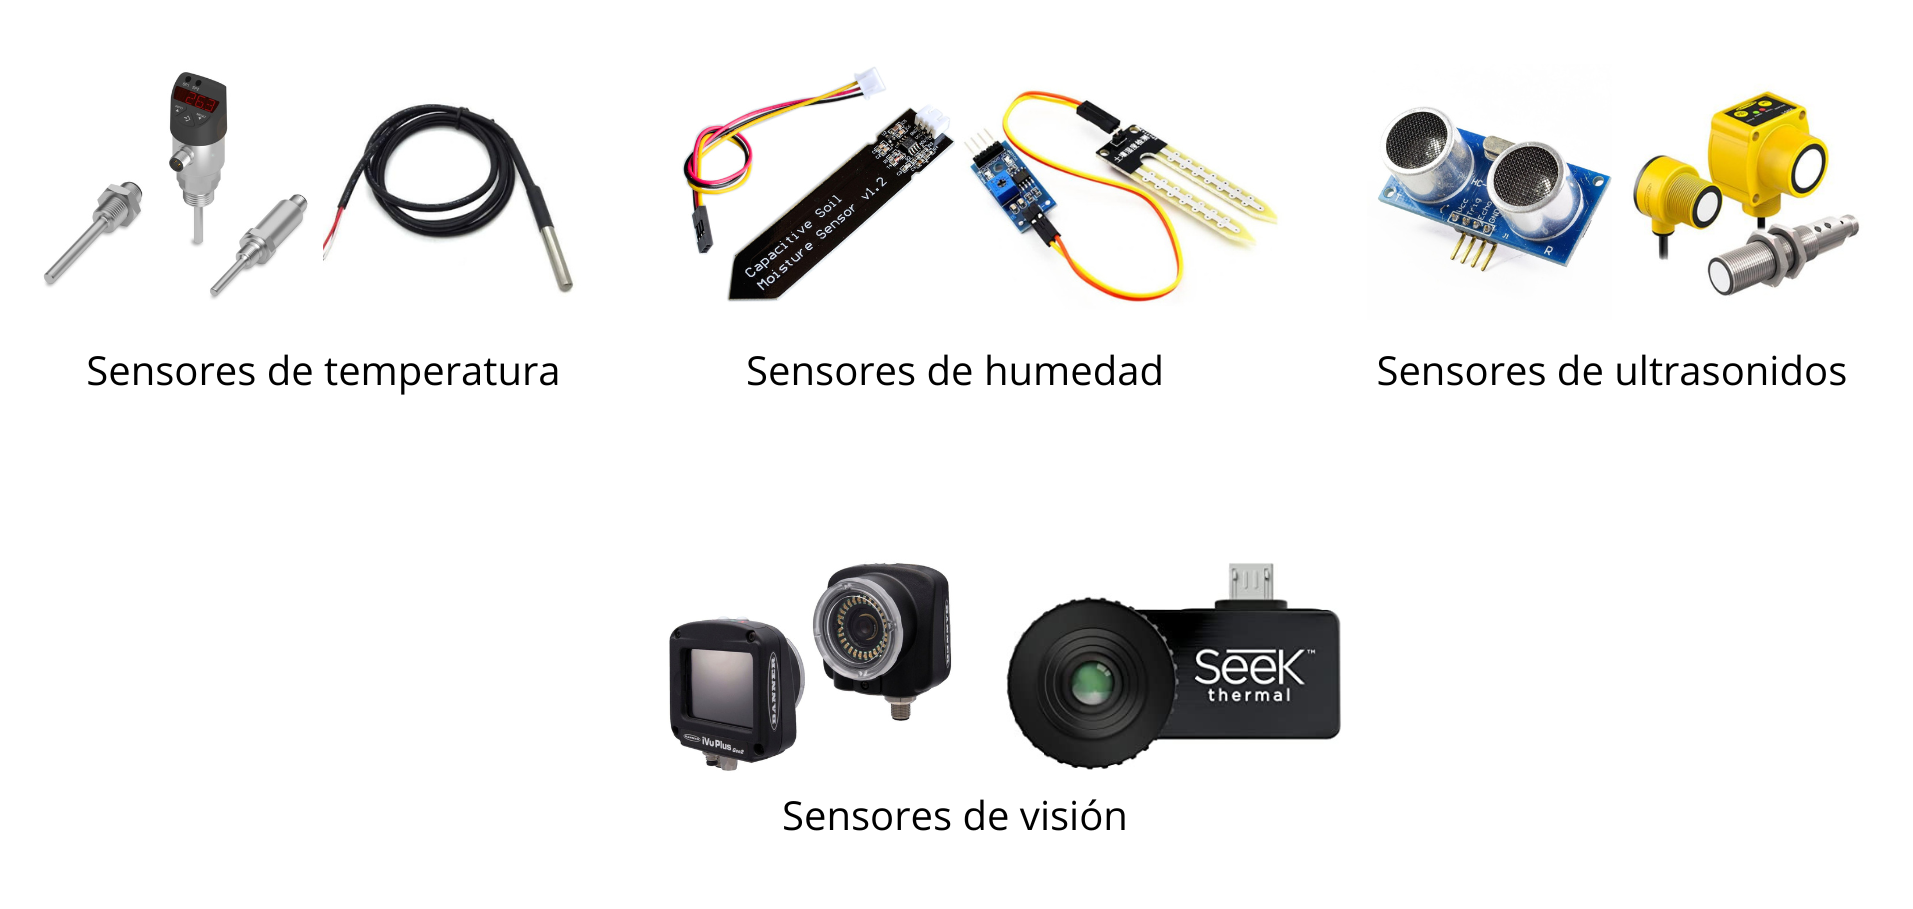
\includegraphics[width=12cm]{figs/sensores}
\end{figure}
\note[item]{Existen distintos tipos de sensores que dotan de distintas cualidades.}
\note[item]{}
\note[item]{Proceso arduo para extraer información útil en tiempo real.}
\note[item]{Para el procesamiento de la información obtenida del sensor de visión, es necesario aplicar un algoritmo de IA.}
\end{frame}

\begin{frame}
\frametitle{Inteligencia Artificial}
\begin{figure}
\centering
\includegraphics[width=7cm]{figs/ia-5}
\end{figure}
\note[item]{La inteligencia artificial consiste en replicar los mecanismos del cerebro mediante algoritmos.}
\note[item]{ Uno de los algoritmos más usados es el ML, preprogramados por un humano y que tratan de descubrir patrones que les hacen aprender.}
\note[item]{Los algoritmos más usados en visión artificial pertenecen a un subcampo del ML denominado DL, donde el autómata aprende por si mismo sin intervención humana, simulando el cerebro con unidades equivalentes a las neuronas.}
\end{frame}

\begin{frame}
\frametitle{Sistemas multisensoriales}
\begin{figure}
\centering
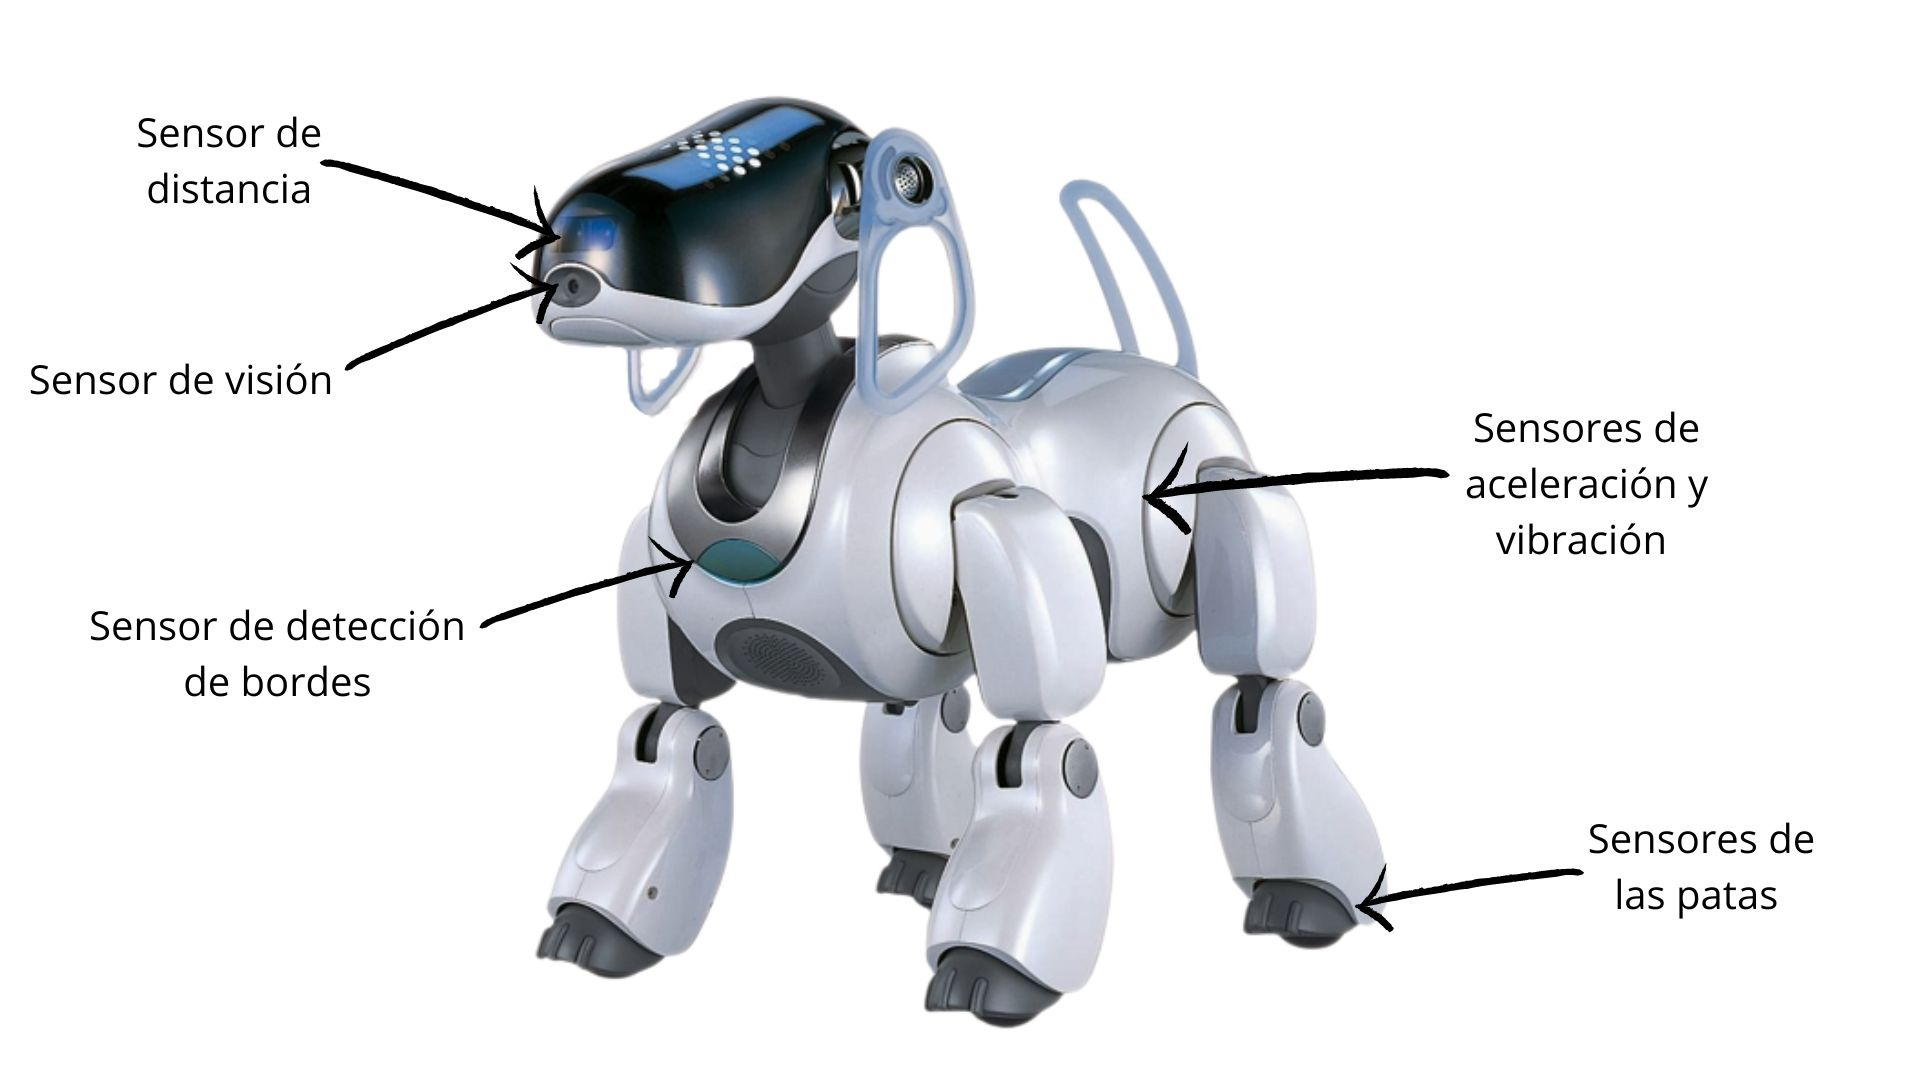
\includegraphics[width=12cm]{figs/multisensorial}
\end{figure}
\note[item]{Además de utilizar sensores de visión, si a un robot se le incorporan diferentes tipos de sensores, este obtendrá mucha más información, por lo que podrá ser más preciso y simular a un humano mejor.}
\note[item]{Este trabajo se enmarca en el contexto de los sistemas multisensoriales, concretamente en los sistemas multisensoriales destinados al bienestar animal y al análisis de comportamiento.}
\end{frame}

%------------------------------------------------------------------------------OBJETIVOS------------------------------------------------------------------------------
\section*{}
\begin{frame}{}
  \centering \Huge
  \emph{Objetivos}
\note[item]{Pasemos ahora a comentar los objetivos que se han marcado con este trabajo.}
\end{frame}

\setbeamercolor{block title}{bg=mypink!40,fg=black}


\section{Objetivos}
\begin{frame}
\begin{block}{Objetivos}
\begin{itemize}
\item Recoger la lectura de los sensores en paralelo en un mismo fichero.
\item Crear un servidor web para los sensores de las cámaras.
\item Detectar los ratones mediante algoritmos de Deep Learning.
\end{itemize}
\end{block}

\begin{block}{Requisitos}
\begin{itemize}
\item El sistema debe ser capaz de ejecutar en tiempo real sobre Raspberry.
\item El lenguaje de programación debe ser Python.
\item La interfaz de usuario se creará en Node-Red.
\end{itemize}
\end{block}
\end{frame}

%---------------------------------------------------------------------------DISEÑO-----------------------------------------------------------------------------
\section*{}
\begin{frame}{}
  \centering \Huge
  \emph{Diseño}
\note[item]{Una vez descritos los objetivos, se presenta la infraestructura y las plataformas utilizadas.}
\note[item]{Este capítulo se divide en dos partes: HW y SW.}
\end{frame}

\section{Plataforma de desarrollo}
\subsection{Infraestructura hardware}
\begin{frame}
\frametitle{Infraestructura hardware}
\begin{figure}
\centering
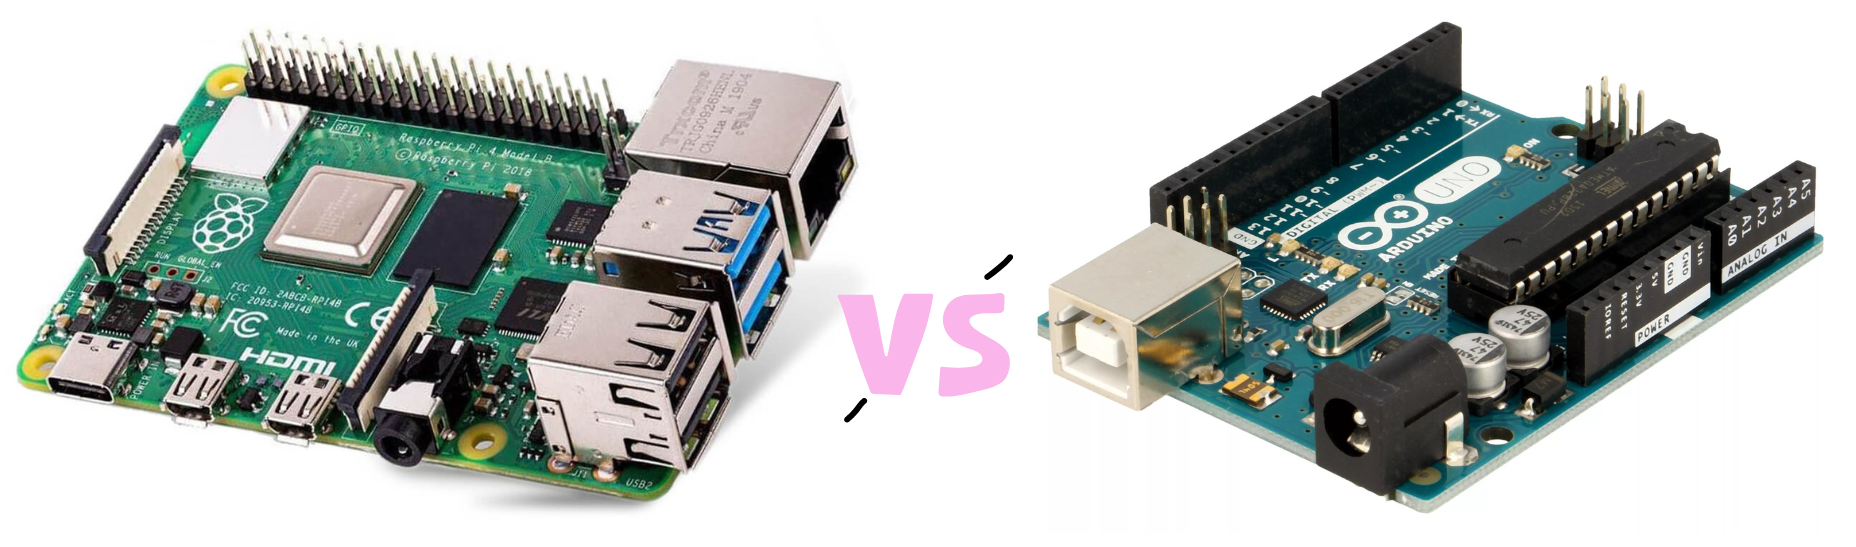
\includegraphics[width=12cm]{figs/VS}
\end{figure}
\begin{multicols}{2}

\begin{itemize}
\centering
\item[] Pines GPIO
\item[] Conexión de cámaras
\item[] Cuatro puertos USB
\item[] Dos puertos micro-USB
\item[] Microordenador
\item[] Sistema operativo completo
\item[] Pines GPIO
\item[] No conexión de cámaras
\item[] No tiene puertos USB
\item[] No tiene puertos micro-USB
\item[] Microprocesador
\item[] IDE
\end{itemize}

\end{multicols}
\note[item]{Comenzando por la infraestructura HW}
\note[item]{Existen distintos sistemas embebidos que se podrían haber utilizado para este trabajo. Los dos más conocidos son Raspberry y Arduino. Hay varias características favorables a Raspberry que han hecho que se seleccione esta placa frente a Arduino.}
\note[item]{ENTORNO DE DESARROLLO INTERACTIVO}
\end{frame}

\subsection{Infraestructura hardware}
\begin{frame}
\begin{figure}
\centering
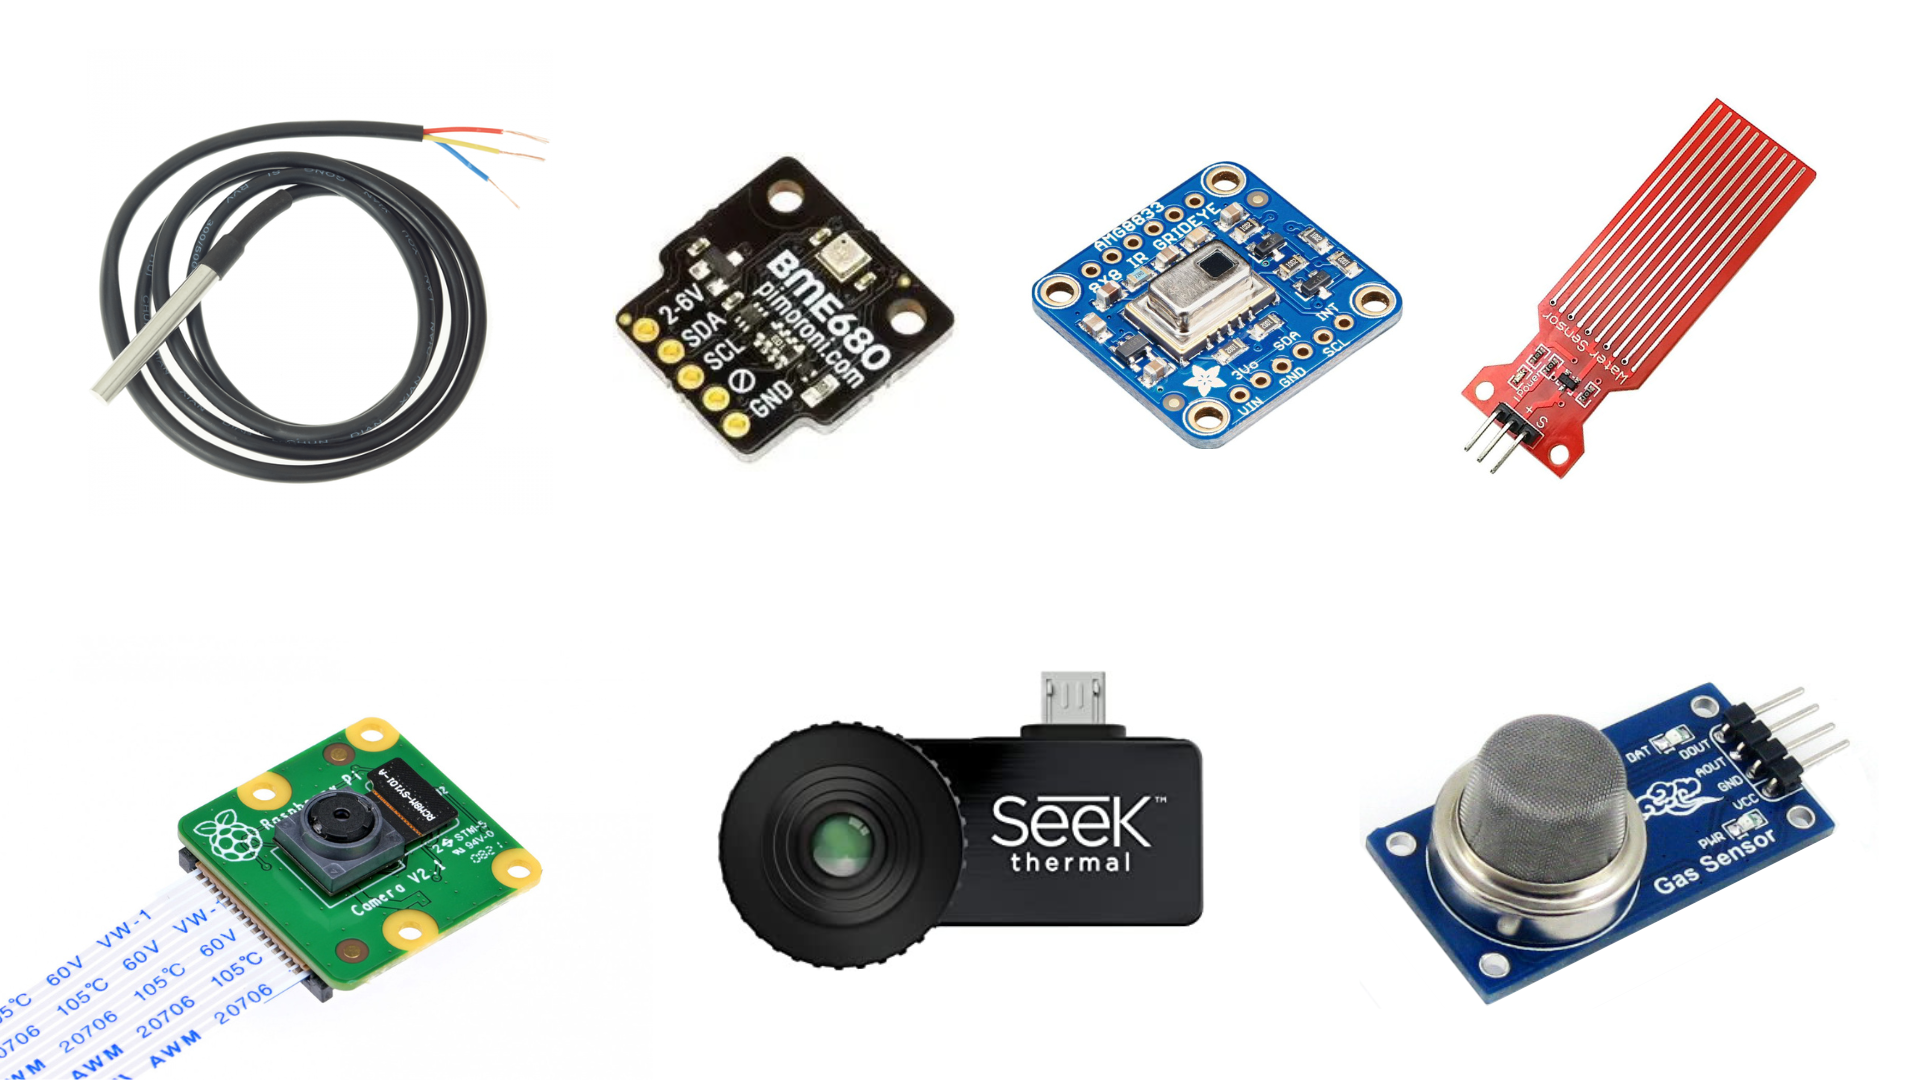
\includegraphics[width=12cm]{figs/sensoresusados}
\end{figure}
\note[item]{A través de los múltiples pines, se han conectado los sensores utilizados para el funcionamiento del sistema.} \note[item]{RESISTENCIA AL AIRE}
\note[item]{CONCENTRACIÓN DE GASES}
\note[item]{A continuación se procede a describir la infraestructura SW, donde se explican las plataformas utilizadas.}
\end{frame}

\subsection{Infraestructura software}
\begin{frame}
\frametitle{Infraestructura software}
\begin{figure}
\centering

\includegraphics[width=10cm]{figs/apps}
\end{figure}
\note[item]{BASADO en Debian}
\note[item]{SOPORTADO DE FORMA NATIVA EN EL SO}
\end{frame}

%-----------------------------------------------------------------------DESARROLLO DEL SISTEMA----------------------------------------------------------------------
\section*{}
\begin{frame}{}
  \centering \Huge
  \emph{Desarrollo del sistema}
\note[item]{A continuación se presenta el desarrollo que se ha llevado a cabo para la obtención del sistema planteado. De nuevo, se divide en desarrollo HW y desarrollo SW.}
\end{frame}

\section{Desarrollo del sistema}
\subsection{Desarrollo hardware}
\begin{frame}
\frametitle{Desarrollo hardware}
Conexión de los sensores a la placa.
\begin{figure}
\centering
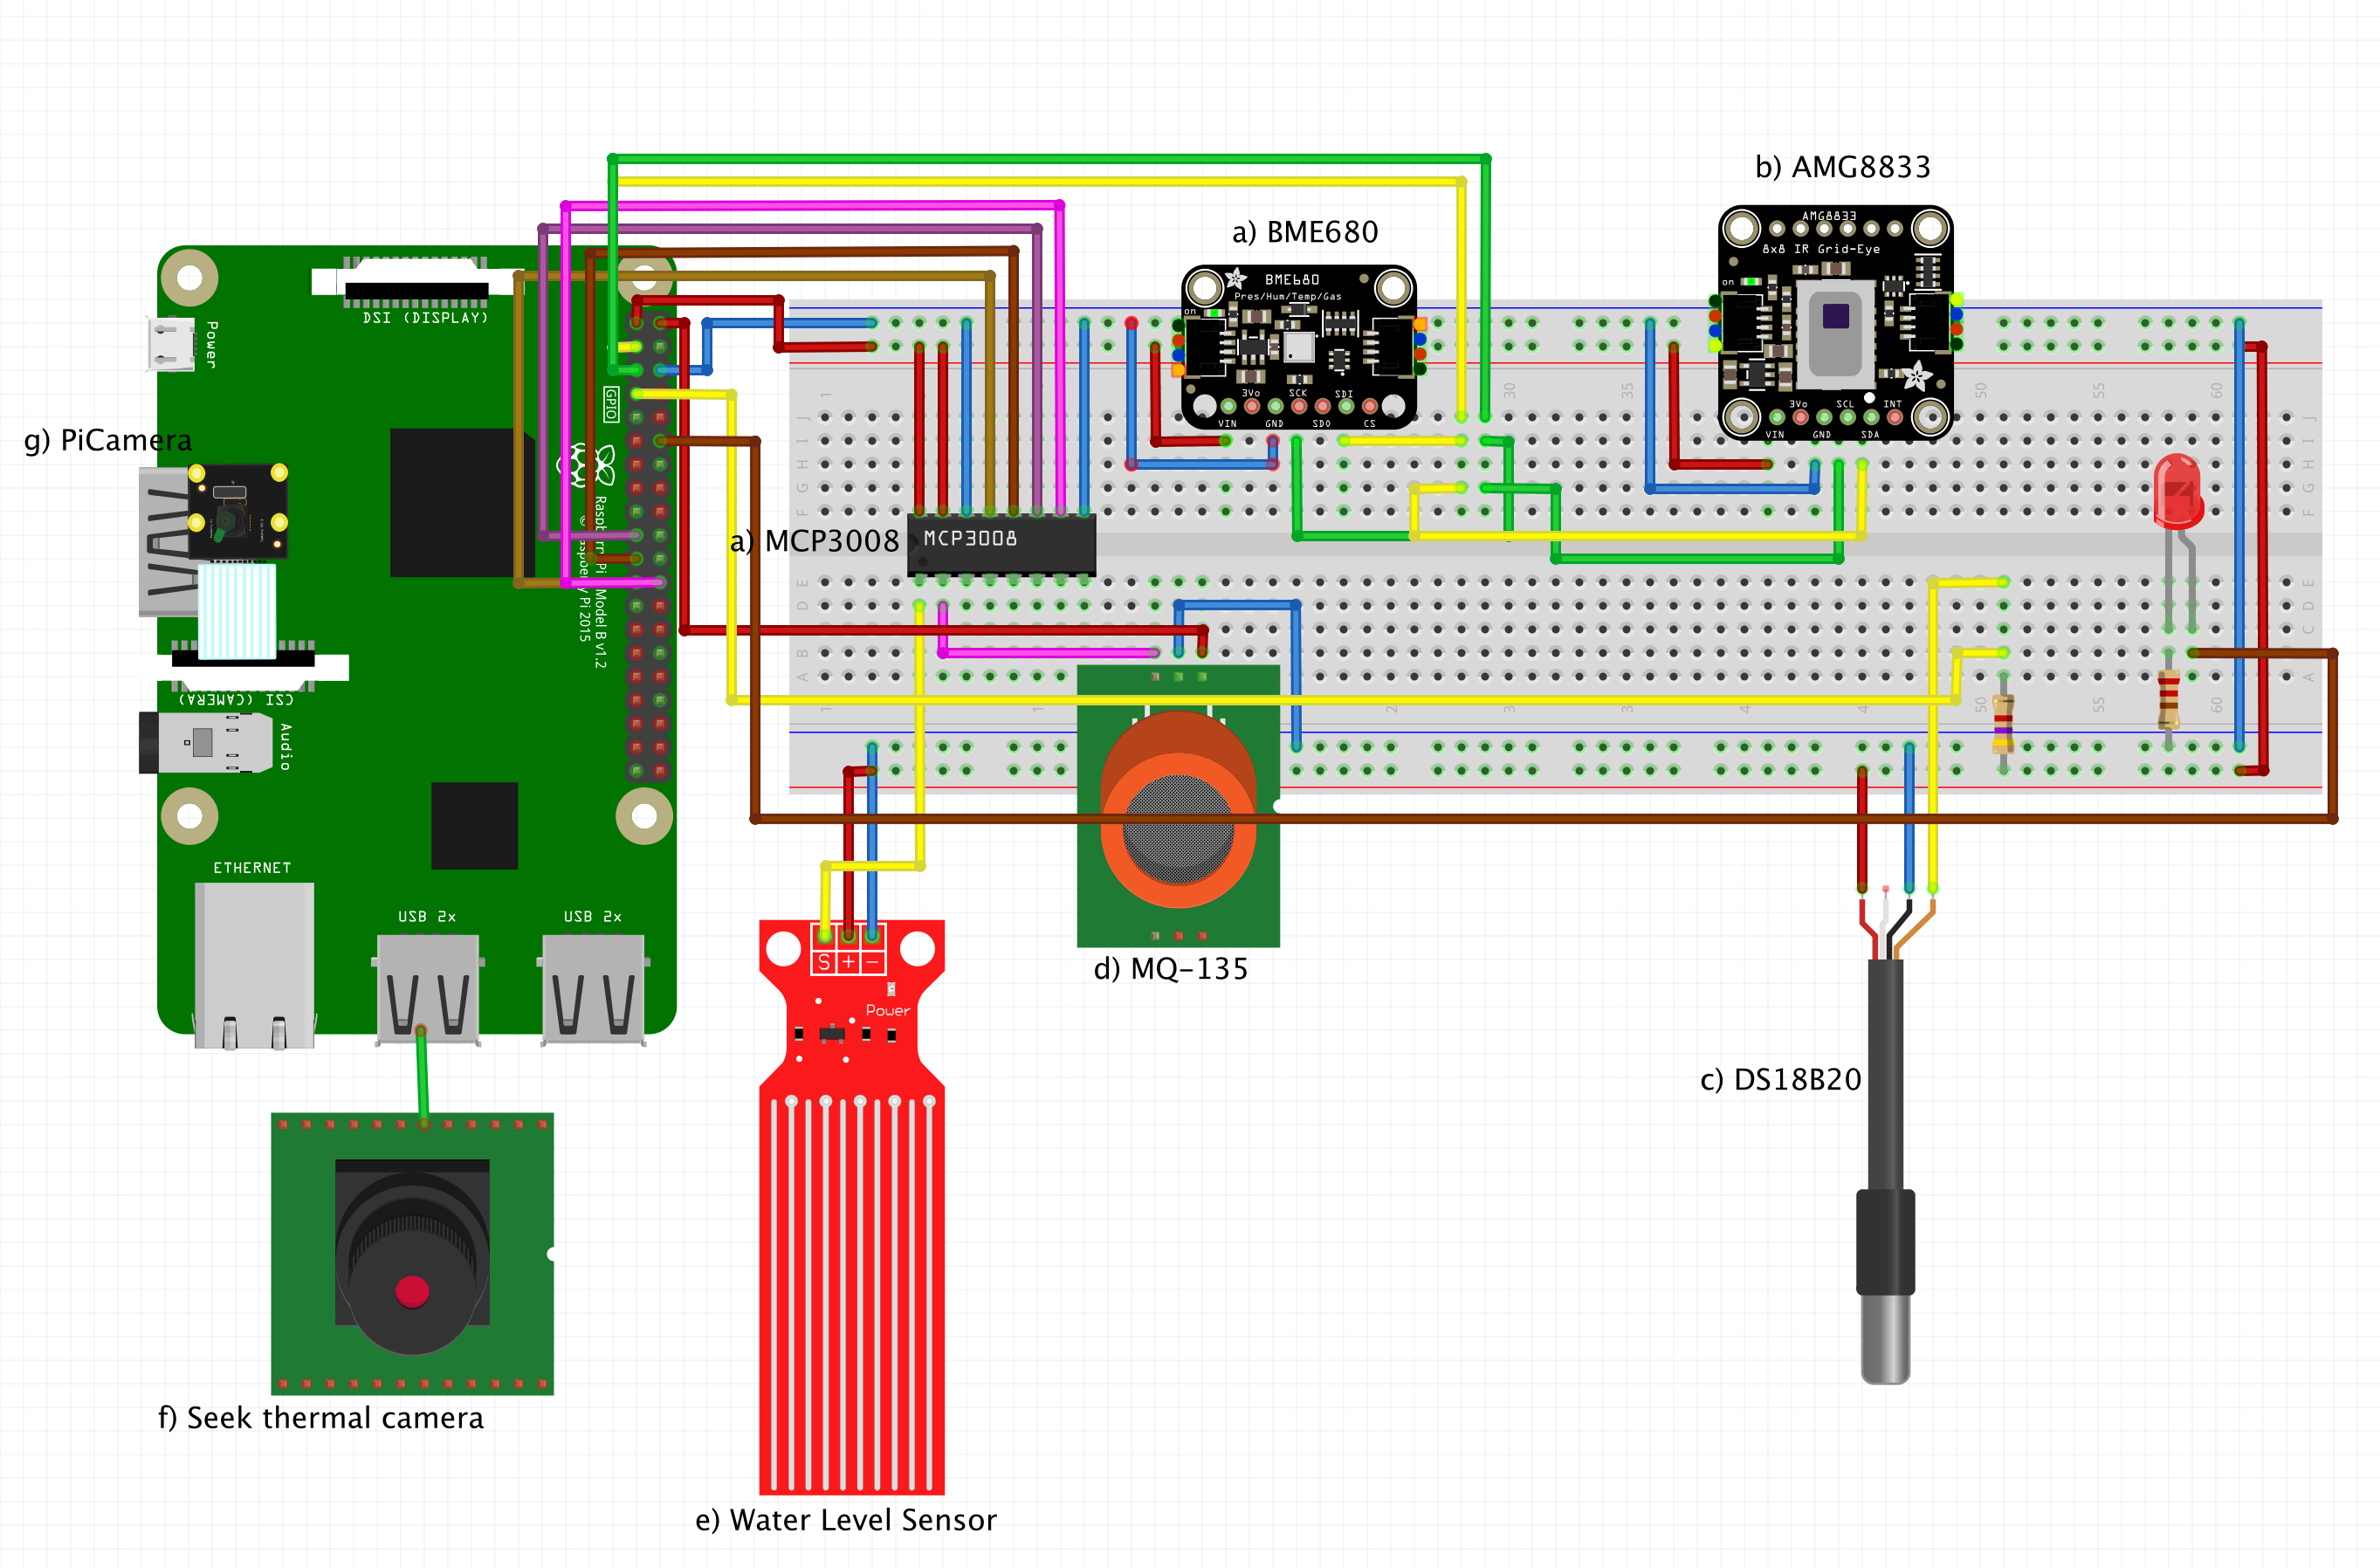
\includegraphics[width=10cm]{figs/conexiones}
\end{figure}
\note[item]{Comenzando con el desarrollo HW, se han conectado los sensores a la placa.}
\end{frame}

\subsection{Desarrollo software}
\begin{frame}
\frametitle{Desarrollo software}
\begin{enumerate}
\item Lectura sensorial con Python
\item Creación de la interfaz de usuario
\item Integración de las cámaras en la IU
\end{enumerate}
\begin{figure}
\centering
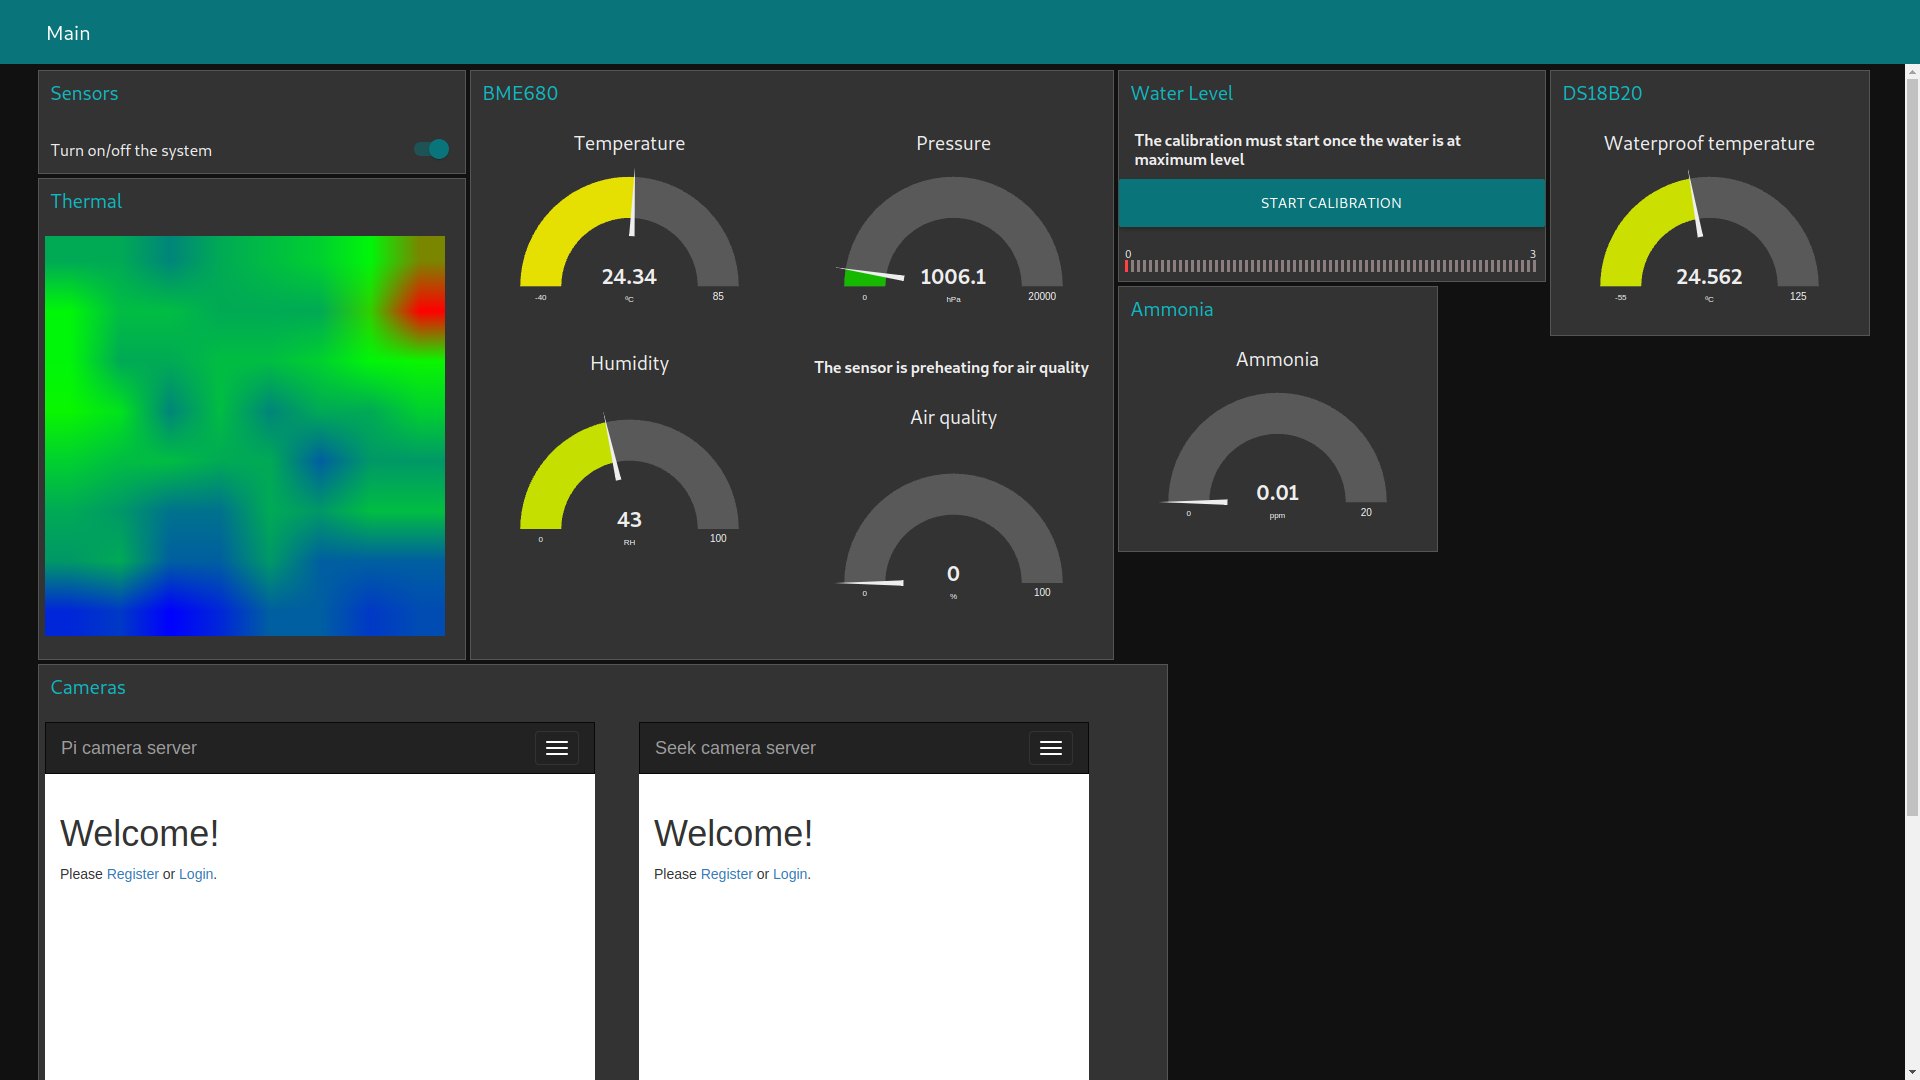
\includegraphics[width=10cm]{figs/UIcompleta}
\end{figure}
\note[item]{Diagrama de casos de uso y diagrama de clases del sistema}
\note[item]{RESISTENCIA AL AIRE --- CALIDAD DEL AIRE}
\end{frame}

\begin{frame}
\frametitle{Seguridad}
\begin{itemize}
\item Servidores con login y 2FA
\item Login en el flujo de Node-Red así como en la interfaz de usuario
\item Cambio de HTTP a HTTPS
\end{itemize}
\note[item]{Todas contraseñas están encriptadas bajo algoritmos de funciones hash en SHA256.}
\end{frame}

\begin{frame}
\frametitle{Autoarranque}
\begin{figure}
\centering
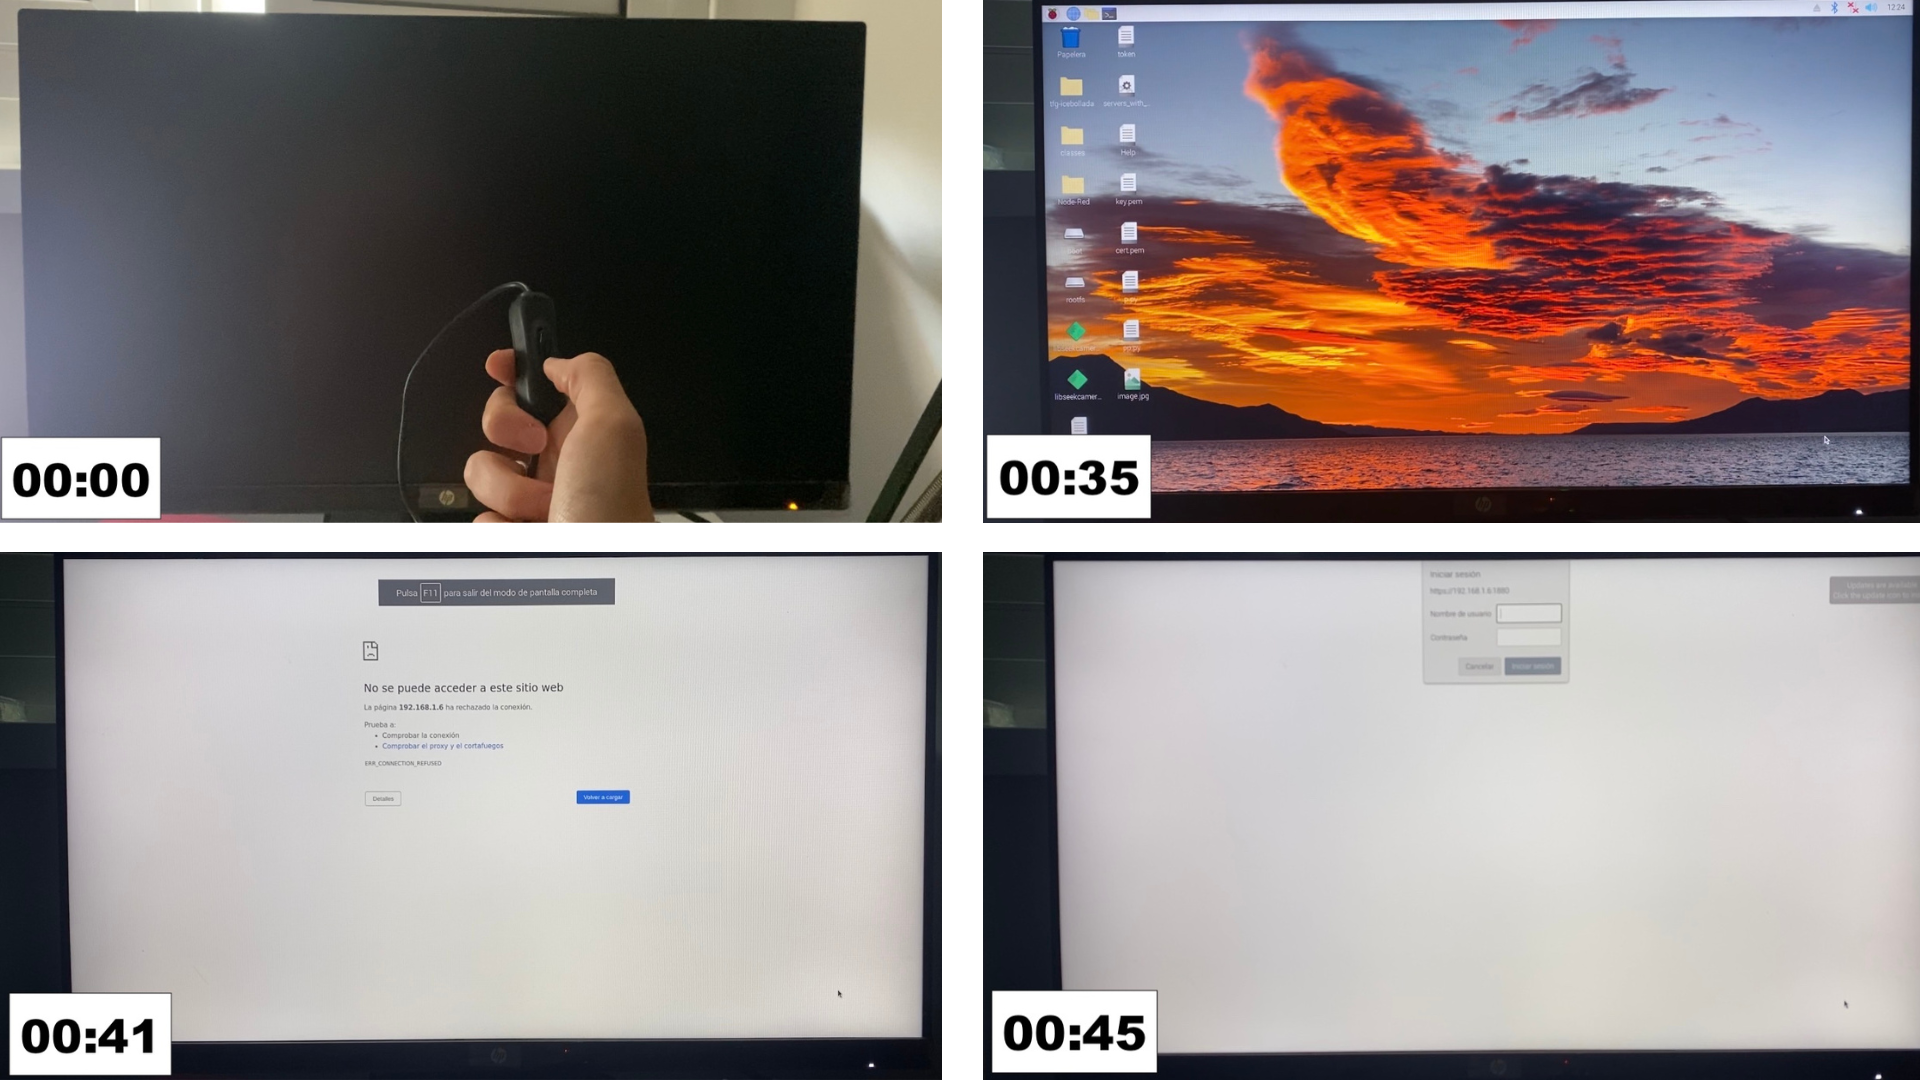
\includegraphics[width=12cm]{figs/autoarranque}
\end{figure}
\note[item]{Por último, se ha adaptado el sistema de acuerdo a uso de un usuario ajeno a cualquier conocimiento de robótica.}
\end{frame}

\begin{frame}
\frametitle{Detección de ratones mediante técnicas de Deep Learning}
\begin{figure}
\centering
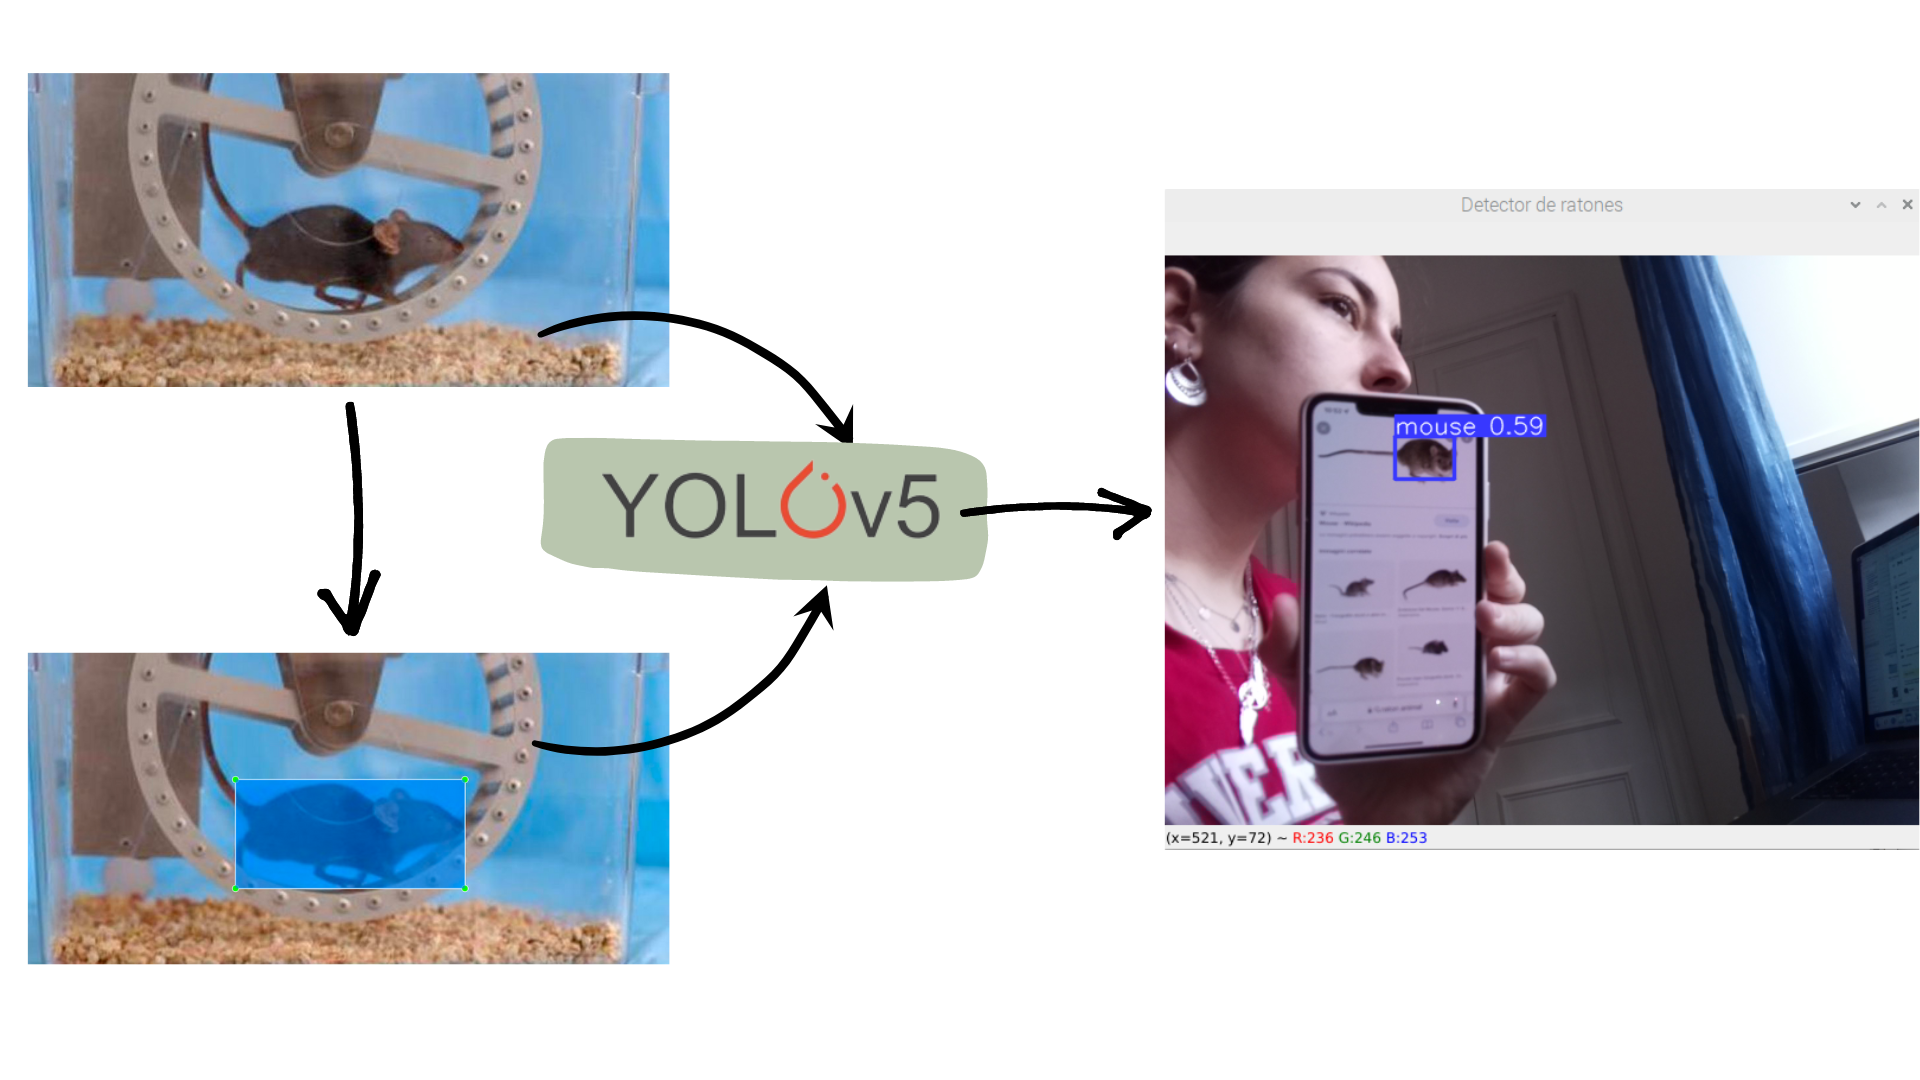
\includegraphics[width=12cm]{figs/deteccion-2}
\end{figure}
\note[item]{354 imágenes: 275 para el proceso de entrenamiento y 79 para el de validación.}
\end{frame}

%-----------------------------------------------------------------------CONCLUSIONES---------------------------------------------------------------------------------------
\section*{}
\begin{frame}{}
  \centering \Huge
  \emph{Conclusiones}
\note[item]{Para acabar esta presentación, vamos a repasar lo hecho, unas breves conclusiones y las líneas futuras.}
\end{frame}

\section{Conclusiones}
\begin{frame}
\frametitle{Conclusiones}
\begin{block}{Objetivos cumplidos}
\begin{itemize}
\item Interfaz de usuario creado en Node-Red .
\item Detección de ratones mediante algoritmo de Deep Learning.
\item El sistema funciona en tiempo real en Raspberry: sistema \textit{low-cost}.
\item Interfaz intuitiva para el usuario final.
\item Accesible desde cualquier dispositivo de la misma red.
\end{itemize}
\note[item]{Se han cumplido los objetivos presentados en el capítulo 2.}
\end{block}

\begin{block}{Líneas futuras}
\begin{itemize}
\item Adaptación de la IU a un servidor accesible desde cualquier lugar.
\item Análisis del comportamiento de los animales con técnicas de DL.
\item Creación de un Docker para la instalación por cualquier usuario.
\end{itemize}
\note[item]{Finalmente, algunas de las líneas futuras para finalizar este trabajo son}
\end{block}
\end{frame}

\begin{frame}[plain]
\large{\titlepage}
\note[item]{Y hasta aquí mi exposición.}
\note[item]{Quedo a disposición del tribunal para cualquier duda que tenga.}
\end{frame}
\endgroup
\end{document}
